\chapter{Mathematical Background}

\minitoc




\section{Probability and Information Theory}


\subsection{Joint, marginal and conditional probability}

Let the $n$ (discrete or continuous) random variables $y_1, \ldots, y_n$ have a joint joint probability probability $p(y_1, \ldots, y_n)$, or $p(\mathbf{y})$ for short\footnote{One can deal with more general cases where the density function does not exist by using the distribution function.}. Technically, one ought to distinguish between probabilities (for discrete variables) and probability densities for continuous variables. Throughout the thesis we commonly use the term `probability' to refer to both. Let us partition the variables in $\mathbf{y}$ into two groups, $\mathbf{y}_A$ and $\mathbf{y}_B$, where $A$ and $B$ are two disjoint sets whose union is the set $\{1, \ldots, n\}$, so that $p(\mathbf{y}) = p(\mathbf{y}_A, \mathbf{y}_B)$. Each group may contain one or more variables.

The \emph{marginal} probability of $\mathbf{y}_A$ is given by
\begin{equation}
	p(\mathbf{y}_A) = \int  p(\mathbf{y}_A, \mathbf{y}_B) \, \mathrm{d}\mathbf{y}_B.
\end{equation}
The integral is replaced by a sum if the variables are discrete valued. Notice that if the set $A$ contains more than one variable, then the marginal probability is itself a joint probability---whether it is referred to as one or the other depends on the context. If the joint distribution is equal to the product of the marginals, then the variables are said to be \emph{independent}, otherwise they are \emph{dependent}.

The \emph{conditional} probability function is defined as
\begin{equation}
	p(\mathbf{y}_A|\mathbf{y}_B) = \frac{p(\mathbf{y}_A, \mathbf{y}_B)}{p(\mathbf{y}_B)},
\end{equation}
defined for $p(\mathbf{y}_B) > 0$, as it is not meaningful to condition on an impossible event. If $\mathbf{y}_A$ and $\mathbf{y}_B$ are independent, then the marginal $p(\mathbf{y}_A)$ and the conditional $p(\mathbf{y}_A|\mathbf{y}_B)$ are equal.

Using the definitions of both $p(\mathbf{y}_A|\mathbf{y}_B)$ and $p(\mathbf{y}_B|\mathbf{y}_A)$ we obtain \emph{Bayes' theorem}:
\begin{equation}
\label{eq:bayes-thm}
	p(\mathbf{y}_A|\mathbf{y}_B) = \frac{p(\mathbf{y}_B|\mathbf{y}_A)p(\mathbf{y}_A)}{p(\mathbf{y}_B)}.
\end{equation}
Since conditional distributions are themselves probabilities, one can use all of the above also when further conditioning on other variables. For example, in supervised learning, one often conditions on the inputs throughout, which would lead e.g.\ to a version of Bayes' rule with additional conditioning on $X$ in all four probabilities in Eq.~\eqref{eq:bayes-thm}.


\subsection{Change of variables}

For a univariate continuous random variable $x$ with distribution $p(x)$, the transformation $y = f(x)$, where $f(x)$ is a monotonic function, has distribution
\begin{equation}
\label{eq:pdf-chg-of-vars}
	p(y) = p(x)\left|\frac{df}{dx}\right|^{-1},
	\qquad x = f^{-1}(y).
\end{equation}
For multivariate $\mathbf{x}$ and bijection $\mathbf{f}(\mathbf{x})$, then $\mathbf{y} = \mathbf{f}(\mathbf{x})$ has distribution
\begin{equation}
\label{eq:pdf-chg-of-vars-multi}
	p(\mathbf{y}) = p(\mathbf{x} = \mathbf{f}^{-1}(\mathbf{y}))\left|\mathrm{det}\left(\frac{\partial \mathbf{f}}{\partial \mathbf{x}}\right)\right|^{-1},
\end{equation}
where the Jacobian matrix has elements
\begin{equation}
	\left[\frac{\partial \mathbf{f}}{\partial \mathbf{x}}\right]_{i,\, j}
	= \frac{\partial f_{i}(\mathbf{x})}{\partial x_j}.
\end{equation}
Sometimes, one needs to consider transformations between different dimensions. For example, if $\mathbf{z}$ has lower dimension than $\mathbf{x}$, then one may introduce additional variables $\mathbf{z}^\prime$ to define a new multivariate $\mathbf{y} = (\mathbf{z},\, \mathbf{z}^\prime)$ with the same dimension as $\mathbf{x}$. Then one applies the transformation \eqref{eq:pdf-chg-of-vars-multi} to give the distribution on the joint variables $\mathbf{y}$, from which $p(\mathbf{z})$ can be obtained by marginalisation.


\subsection{Entropy and Kullback-Leibler divergence}
\label{sec:entropy}

The \emph{entropy} $\mathrm{H}[p(\mathbf{x})]$ of a distribution $p(\mathbf{x})$ is a non-negative measure of the amount of `uncertainty' in the distribution, and is defined as
\begin{equation}
	\mathrm{H}[p(\mathbf{x})] \equiv -\int p(\mathbf{x})\log p(\mathbf{x}) \, \mathrm{d}\mathbf{x}.
\end{equation}
The integral is substituted by a sum for discrete variables. Entropy is measured in \emph{bits} if the log is to the base 2 and in \emph{nats} in the case of the natural log.

The Kullback-Leibler (KL) divergence (or relative entropy) $\mathrm{KL}(p \Vert q)$ between two distributions $p(\mathbf{x})$ and $q(\mathbf{x})$ is defined as
\begin{equation}
	\mathrm{KL}(p \Vert q) = \int p(\mathbf{x})\log\frac{p(\mathbf{x})}{q(\mathbf{x})} \, \mathrm{d}\mathbf{x}.
\end{equation}
It is easy to show that $\mathrm{KL}(p \Vert q) \geq 0$, with equality if $p = q$ (almost everywhere). The KL divergence can be viewed as the extra number of nats needed on average to code data generated from a source $p(\mathbf{x})$ under the distribution $q(\mathbf{x})$ as opposed to $p(\mathbf{x})$.




\section{Convex Optimisation}

In this section, we give a gentle introduction to convex optimisation and present some basic algorithms for solving convex mathematical programs. A broad and significantly more detailed literature exists, and the reader is referred to \cite{nemirovski, rockafellar, fletcher, bv_cvxbook, borwein, bubeck}, among others. We give here only the most elementary analysis, and focus on the techniques that are of use to us throughout the thesis.

\subsection{Basic definitions and setup}
\label{sec:cvxopt-defs}

The goal in this chapter is to minimise a continuous and convex function over a convex subset of the Euclidean space. Henceforth, let $\mathcal{K} \subseteq \mathbb{R}^d$ be a bounded, convex and compact set in the Euclidean space. 
\begin{mydef}
\label{def:diameter}
The \emph{diameter} of $\mathcal{K}$ is defined as
\begin{equation}
\mathrm{diam}(\mathcal{K}) \equiv \sup_{\mathbf{x}, \mathbf{y} \in \mathcal{K}} \, \Vert\mathbf{x} - \mathbf{y}\Vert_2,
\end{equation}
where $\Vert\mathbf{x}\Vert_2 = \sqrt{\mathbf{x}\cdot\mathbf{x}}$ is the Euclidean norm.
\end{mydef}
%We denote by $D$ an upper bound on the diameter of $\mathcal{K}$:
%\begin{equation}
%\forall \mathbf{x}, \mathbf{y} \in \mathcal{K},
%\Vert\mathbf{x} − \mathbf{y}\Vert_2 \leq D.
%\end{equation}
\begin{mydef}
\label{def:convex-set}
A set $\mathcal{K}$ is \emph{convex} if for any $\mathbf{x}, \mathbf{y} \in \mathcal{K}$, all the points on the line segment connecting $\mathbf{x}$ and $\mathbf{y}$ also belong to $\mathcal{K}$, i.e.\
\begin{equation}
\forall \alpha \in [0, 1], \quad \alpha\mathbf{x} + (1-\alpha)\mathbf{y} \in \mathcal{K}. 
\end{equation}
\end{mydef}
\begin{mydef}
\label{def:convex-function}
A function $f:\mathcal{K} \rightarrow \mathbb{R}$ is \emph{convex} if for any $\mathbf{x}, \mathbf{y} \in \mathcal{K}$,
\begin{equation}
\forall \alpha \in [0, 1], \quad f[(1-\alpha)\mathbf{x} + \alpha\mathbf{y}] \leq (1-\alpha)f(\mathbf{x}) + \alpha f(\mathbf{y}).
\end{equation}
Equivalently, if $f(\cdot)$ is differentiable, that is, its gradient $\nabla f(\mathbf{x})$ exists for all $\mathbf{x} \in \mathcal{K}$, then it is convex if and only if $\forall\mathbf{x}, \mathbf{y} \in \mathcal{K}$,
\begin{equation}
\label{eq:convex-function}
f(\mathbf{y}) \geq f(\mathbf{x}) + \nabla f(\mathbf{x}) \cdot(\mathbf{y} - \mathbf{x}).
\end{equation}
\end{mydef}
\begin{mydef}
\label{def:subgradient}
For convex and non-differentiable functions $f(\cdot)$, the \emph{subgradient} of $f(\cdot)$ at $\mathbf{x}$ is defined to be any vector $\mathbf{z}$ that satisfies the inequality
\begin{equation}
f(\mathbf{y}) \geq f(\mathbf{x}) + \mathbf{z}\cdot(\mathbf{y} - \mathbf{x}),
\end{equation}
for all $\mathbf{y} \in \mathcal{K}$. We call \emph{subdifferential set} the set of subgradients of $f(\cdot)$ at $\mathbf{x}$, and denote it as $\partial f(\mathbf{x})$. Furthermore, if $f(\cdot)$ is differentiable at $\mathbf{x}$, then $\partial f(\mathbf{x})$ contains a single element, namely the gradient $\nabla f(\mathbf{x})$ of $f(\cdot)$ at $\mathbf{x}$.
\end{mydef}

We denote by $G > 0$ an upper bound on the norm of the subgradients of $f(\cdot)$ over $\mathcal{K}$, i.e.\ $\Vert \nabla f(\mathbf{x})\Vert_2 \leq G$ for all $\mathbf{x} \in \mathcal{K}$. Such an upper bound implies that the function $f(\cdot)$ is Lipschitz continuous with parameter $G$.
\begin{mydef}
\label{def:lipschitz-continuity}
The function $f:\mathcal{K} \rightarrow \mathbb{R}$ is said to be \emph{Lipschitz continuous} with constant $G > 0$ if for all $\mathbf{x}, \mathbf{y} \in \mathcal{K}$, we have
\begin{equation}
|f(\mathbf{x}) - f(\mathbf{y})| \leq G\Vert\mathbf{x} - \mathbf{y}\Vert_2.
\end{equation}
\end{mydef}
The optimisation and machine learning communities study special types of convex functions that admit useful properties, which in turn allow for more efficient optimisation. Below, we define the most notable of these properties.
\begin{mydef}
\label{def:strongly-convex-function}
We say that a function $f : \mathcal{K} \rightarrow \mathbb{R}$ is $\lambda$-\emph{strongly convex} if
\begin{equation}
f(\mathbf{y}) \geq f(\mathbf{x}) + \nabla f(\mathbf{x})\cdot(\mathbf{y} - \mathbf{x}) + \frac{\lambda}{2}\Vert\mathbf{y} - \mathbf{x}\Vert_2^2,
\qquad \forall \, \mathbf{x}, \mathbf{y} \in \mathcal{K}.
\end{equation}
\end{mydef}
\begin{mydef}
\label{def:smooth-function}
A function $f : \mathcal{K} \rightarrow \mathbb{R}$ is $L$-\emph{smooth} if
\begin{equation}
f(\mathbf{y}) \leq f(\mathbf{x}) + \nabla f(\mathbf{x})\cdot(\mathbf{y} - \mathbf{x}) + \frac{L}{2}\Vert\mathbf{y} - \mathbf{x}\Vert_2^2,
\qquad \forall \, \mathbf{x}, \mathbf{y} \in \mathcal{K}.
\end{equation}
The latter condition is equivalent to the Lipschitz continuity of the gradients of $f(\cdot)$, with Lipschitz constant $L > 0$, i.e.\
\begin{equation}
\Vert\nabla f(\mathbf{x}) - \nabla f(\mathbf{y})\Vert_2 \leq L\Vert\mathbf{x} - \mathbf{y}\Vert_2,
\qquad \forall \, \mathbf{x}, \mathbf{y} \in \mathcal{K}.
\end{equation}
\end{mydef}
Throughout the thesis, we refer to $\lambda$-strongly convex functions simply as strongly convex functions. Similarly, we shall call smooth functions those functions satisfying Definition~\ref{def:smooth-function}.

If the function is twice-differentiable and admits a second derivative, known as the Hessian for a function of several variables, Definitions~\ref{def:strongly-convex-function} and~\ref{def:smooth-function} are equivalent to the following condition on the Hessian, which we denote by $\nabla^2 f(\mathbf{x})$:
\begin{equation}
\alpha\mathbf{I} \preceq \nabla^2 f(\mathbf{x}) \preceq \beta\mathbf{I},
\end{equation}
where $A \preceq B$ means the matrix $B - A$ is positive semi-definite.

When the function $f(\cdot)$ is both strongly convex and smooth, we say that it is $\gamma$-well-conditioned, where $\gamma$ is the ratio between strong convexity and smoothness, and is also known as the \emph{condition number} of $f(\cdot)$:
\begin{equation}
\gamma = \frac{\lambda}{L} \leq 1.
\end{equation}
\begin{example}
 The following functions are both strongly convex and smooth:
\begin{enumerate}
	\item A quadratic form $f(\mathbf{x}) = \mathbf{x}^\top A \mathbf{x} - 2\mathbf{b}^\top\mathbf{x}$, where $a\mathbf{I} \preceq A \preceq b\mathbf{I}$, for $a > 0$ and $b < \infty$;
	\item The regularised logistic loss $f(\mathbf{x}) = \log[1 + \exp(\mathbf{b}^\top\mathbf{x})] + \frac{\lambda}{2}\Vert\mathbf{x}\Vert_2^2$, where $\lambda > 0$.
\end{enumerate}
\end{example}

\subsection{Projections onto convex sets}
\label{sec:euclidean-projections}

Throughout the thesis, we shall make use of a projection operation onto a convex set, which is defined as the closest point inside that set to a given point. Formally:
\begin{equation}
  \Pi_\mathcal{K}(\mathbf{y})
  \equiv \, \argmin_{\mathbf{x} \in \mathcal{K}} \Vert \mathbf{x} - \mathbf{y} \Vert_2.
\end{equation}  
When clear from the context, we shall omit the $\mathcal{K}$ subscript. It is left as an exercise to the reader to prove that the projection of a given point over a compact convex set exists and is unique.

The computational complexity of projections is a subtle issue that depends much on the characterisation of $\mathcal{K}$ itself. Most generally, $\mathcal{K}$ can be represented by a membership oracle---an efficient procedure that is capable of deciding whether a given $\mathbf{x}$ belongs to $\mathcal{K}$ or not. In this case, projections can be computed in polynomial time. In certain special cases, projections can be computed very efficiently in near-linear time. A crucial property of projections that we shall make extensive use of is Pythagoras' theorem, which we state below for completeness.
\begin{theorem}[Pythagoras, circa 500 BC]
  \label{thm:pythagoras}
  Let $\mathcal{K} \subseteq \mathbb{R}^d$ be a convex set, $\mathbf{y} \in \mathbb{R}^d$ and $\mathbf{x} = \Pi_\mathcal{K}(\mathbf{y})$. Then, for any $\mathbf{z} \in \mathcal{K}$, we have
  \begin{equation}
    \Vert \mathbf{y} - \mathbf{z} \Vert_2 \geq \Vert \mathbf{x} - \mathbf{z} \Vert_2.
  \end{equation}
\end{theorem}
\begin{figure}[t]
\centering
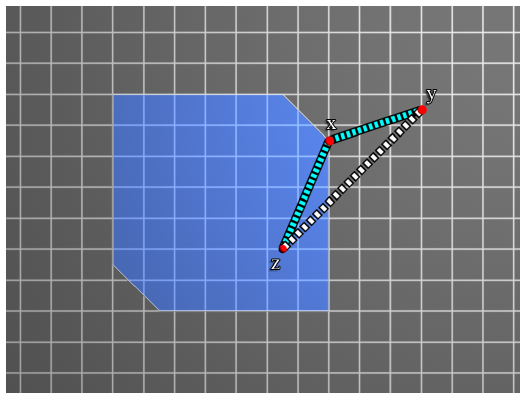
\includegraphics[scale=0.7]{pythagoras}
\caption{An illustration of Pythagoras' theorem. Source: \citep{oco}.}
\label{fig:pythagoras}
\end{figure}
We note that there exists a more general version of Pythagoras' theorem. The above theorem and the definition of projections are true and valid not only for Euclidean norms, but for any norm. In addition, projections according to other distances that are not norms can be defined, in particular with respect to Bregman divergences, and an analogue of Pythagoras' theorem remains valid in such cases.

\subsection{Introduction to optimality conditions}

The standard curriculum of high-school mathematics contains the basic facts about when a function (usually in one dimension) attains a local optimum or saddle point. The generalisation of these conditions to multiple dimensions is called the Karush-Kuhn-Tucker (KKT) conditions, and the reader is referred to \cite{nemirovski, rockafellar, fletcher, bv_cvxbook, borwein, bubeck} for an in-depth rigorous discussion of optimality conditions in general mathematical programming.

We shall only describe briefly and intuitively the main facts that are useful for our purposes. Naturally, we restrict ourselves to convex programming, and thus a local minimum of a convex univariate function is also a global minimum (because the second derivative of a convex function is non-negative everywhere).

The generalisation of the fact that a minimum of a convex differentiable function on $\mathbb{R}$ is a point in which its derivative is equal to zero is given by the multi-dimensional analogue that its gradient is equal to the zero vector:
\begin{equation}
\nabla f(\mathbf{x}) = \mathbf{0}_{d\times 1} \quad \iff \quad \mathbf{x} \in \argmin_{\mathbf{x} \in \mathbb{R}^d} \, f(\mathbf{x}). 
\end{equation}

We will require a slightly more general, but equally intuitive, fact for constrained optimisation: at a minimum point of a constrained convex function, the inner product between the negative gradient and direction towards the interior of $\mathcal{K}$ is non-positive. This is depicted in Figure~\ref{fig:optimality-conditions}, which shows that $-\nabla f(\mathbf{x}^*)$ defines a supporting hyperplane to $\mathcal{K}$. The intuition is that if the inner product were positive, one could improve the objective by moving in the direction of the projected negative gradient. This fact is stated formally in the following theorem.
\begin{figure}[t]
\centering
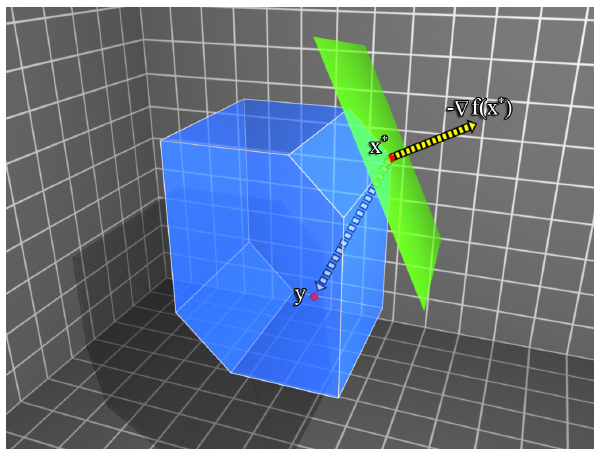
\includegraphics[scale=0.7]{optimality-conditions}
\caption{Optimality conditions: negative gradient pointing outwards. Source: \citep{oco}.}
\label{fig:optimality-conditions}
\end{figure}
\begin{theorem}[Karush-Kuhn-Tucker]
\label{thm:kkt}
Let $\mathcal{K} \subseteq \mathbb{R}^d$ be a convex set, $\mathbf{x}^* \in \argmin_{\mathbf{x} \in \mathcal{K}} \, f(\mathbf{x})$. Then, for any $\mathbf{y} \in \mathcal{K}$, we have
\begin{equation}
\nabla f(\mathbf{x}^*) \cdot (\mathbf{y} - \mathbf{x}^*) \geq 0.
\end{equation}
\end{theorem}


%\section{Gaussian Identities}
%\label{sec:gaussian-identities}
%
%The following identities \citep{rasmussen06} are almost indispensable when dealing with Gaussian distributions, which we denote in the usual way as
%\begin{equation}
%\label{eq:gaussian-pdf-def}
%	\mathcal{N}(\mathbf{x}|\boldsymbol{\mu},\, \boldsymbol{\Sigma})
%	\equiv \frac{1}{\sqrt{|2\pi\boldsymbol{\Sigma}|}}\exp\Big\{-\frac{1}{2}(\mathbf{x} - \boldsymbol{\mu})^\text{T}\boldsymbol{\Sigma}^{-1}(\mathbf{x} - \boldsymbol{\mu})\Big\}.
%\end{equation}
%
%\subsection{Completing the square}
%
%A useful technique in manipulating Gaussians is the so-called technique of `completing the square'. For example, the expression
%\begin{equation}
%	\exp\Big\{-\frac{1}{2}\mathbf{x}^\text{T}\mathbf{A}\mathbf{x} + \mathbf{b}^\text{T}\mathbf{x}\Big\}
%\end{equation}
%can be transformed as follows. First, we complete the square with respect to $\mathbf{x}$ in the exponent:
%\begin{equation}
%	\frac{1}{2}\mathbf{x}^\text{T}\mathbf{A}\mathbf{x} - \mathbf{b}^\text{T}\mathbf{x}
%	= \frac{1}{2}(\mathbf{x} - \mathbf{A}^{-1}\mathbf{b})^\text{T}\mathbf{A}(\mathbf{x} - \mathbf{A}^{-1}\mathbf{b}) - \frac{1}{2}\mathbf{b}^\text{T}\mathbf{A}^{-1}\mathbf{b}.
%\end{equation}
%Hence,
%\begin{equation}
%	\exp\Big\{-\frac{1}{2}\mathbf{x}^\text{T}\mathbf{A}\mathbf{x} + \mathbf{b}^\text{T}\mathbf{x}\Big\}
%	= \mathcal{N}(\mathbf{x}|\mathbf{A}^{-1}\mathbf{b},\, \mathbf{A}^{-1})\sqrt{|2\pi\mathbf{A}^{-1}|}\exp\Big\{\frac{1}{2}\mathbf{b}^\text{T}\mathbf{A}^{-1}\mathbf{b}\Big\}.
%\end{equation}
%From this, one can derive
%\begin{equation}
%	\int \exp\Big\{-\frac{1}{2}\mathbf{x}^\text{T}\mathbf{A}\mathbf{x} + \mathbf{b}^\text{T}\mathbf{x}\Big\}\,\mathrm{d}\mathbf{x}
%	= \sqrt{|2\pi\mathbf{A}^{-1}|}\exp\Big\{\frac{1}{2}\mathbf{b}^\text{T}\mathbf{A}^{-1}\mathbf{b}\Big\}.
%\end{equation}
%
%\subsection{Product of two Gaussians}
%
%The product of two Gaussians is another Gaussian, with a multiplicative factor:
%\begin{equation}
%\label{eq:product-of-2-gaussians}
%	\mathcal{N}(\mathbf{x}|\boldsymbol{\mu}_1,\, \boldsymbol{\Sigma}_1)\,\mathcal{N}(\mathbf{x}|\boldsymbol{\mu}_2,\, \boldsymbol{\Sigma}_2)
%	= \mathcal{N}(\mathbf{x}|\boldsymbol{\mu},\, \boldsymbol{\Sigma})\frac{\exp\big\{-\frac{1}{2}(\boldsymbol{\mu}_1 - \boldsymbol{\mu}_2)^\text{T}\mathbf{S}^{-1}(\boldsymbol{\mu}_1 - \boldsymbol{\mu}_2)\big\}}{\sqrt{|2\pi\mathbf{S}|}},
%\end{equation}
%where $\mathbf{S} \equiv \boldsymbol{\Sigma}_1 + \boldsymbol{\Sigma}_2$ and the mean and covariance are given by
%\begin{equation}
%	\boldsymbol{\mu}
%	= \boldsymbol{\Sigma}(\boldsymbol{\Sigma}_1^{-1}\boldsymbol{\mu}_1 + \boldsymbol{\Sigma}_2^{-1}\boldsymbol{\mu}_2)
%	\qquad \text{and} \qquad
%	\boldsymbol{\Sigma}
%	= (\boldsymbol{\Sigma}_1^{-1} + \boldsymbol{\Sigma}_2^{-1})^{-1}.
%\end{equation}
%Note that the resulting Gaussian has a precision (inverse covariance) equal to the sum of the precisions, and a mean equal to the convex sum of the means, weighted by the precisions.
%
%To prove Eq. \eqref{eq:product-of-2-gaussians}, simply write out the (lengthy) expressions by using the definition \eqref{eq:gaussian-pdf-def} of the Gaussian PDF, and expanding the terms inside the exponential to verify equality (hint: it may be helpful to expand $\boldsymbol{\Sigma}$ using the matrix inversion lemma in Eq. \eqref{eq:woodbury-identity}) 
%
%\subsection{Affine transformations}
%
%Any affine transformation of a Gaussian random vector is itself Gaussian. More precisely, if $\mathbf{y} \equiv \mathbf{A}\mathbf{x} + \mathbf{b}$ and $\mathbf{x} \sim \mathcal{N}(\mathbf{x}|\boldsymbol{\mu},\, \boldsymbol{\Sigma})$, where $\mathbf{x}$ is an $n$-dimensional column vector, $\mathbf{A}$ is a constant $m\times n$ matrix and $\mathbf{b}$ is an $m\times 1$ vector of constants, then $\mathbf{y}$ has multivariate Gaussian distribution with mean $\mathbf{A}\boldsymbol{\mu} + \mathbf{b}$ and covariance $\mathbf{A}\boldsymbol{\Sigma}\mathbf{A}^\text{T}$. In other words,
%\begin{equation}
%	\mathbf{x} \sim \mathcal{N}(\mathbf{x}|\boldsymbol{\mu},\, \boldsymbol{\Sigma})
%	\quad \implies \quad
%	\mathbf{y} \equiv \mathbf{A}\mathbf{x} + \mathbf{b}
%	\sim \mathcal{N}(\mathbf{y}|\mathbf{A}\boldsymbol{\mu} + \mathbf{b},\, \mathbf{A}\boldsymbol{\Sigma}\mathbf{A}^\text{T}).
%\end{equation}
%
%\subsection{Marginal and conditional Gaussians}
%
%Given a marginal Gaussian distribution for $\mathbf{x}$ and a conditional Gaussian distribution for $\mathbf{y}$ given $\mathbf{x}$ in the form
%\begin{align}
%	p(\mathbf{x}) &= \mathcal{N}(\mathbf{x}|\boldsymbol{\mu},\, \boldsymbol{\Lambda}^{-1})
%	\\
%	p(\mathbf{y}|\mathbf{x}) &= \mathcal{N}(\mathbf{y}|\mathbf{A}\mathbf{x} + \mathbf{b},\, \mathbf{L}^{-1})
%\end{align}
%the marginal distribution of $\mathbf{y}$ and the conditional distribution for $\mathbf{x}$ given $\mathbf{y}$ are given by
%\begin{align}
%	p(\mathbf{y}) &= \mathcal{N}(\mathbf{y}|\mathbf{A}\boldsymbol{\mu} + \mathbf{b},\, \mathbf{L}^{-1} + \mathbf{A}\boldsymbol{\Lambda}^{-1}\mathbf{A}^\text{T})
%	\\
%	p(\mathbf{x}|\mathbf{y}) &= \mathcal{N}(\mathbf{x}|\boldsymbol{\Sigma}\{\mathbf{A}^\text{T}\mathbf{L}(\mathbf{y} - \mathbf{b}) + \boldsymbol{\Lambda}\boldsymbol{\mu}\},\, \boldsymbol{\Sigma})
%\end{align} 
%where
%\begin{equation}
%	\boldsymbol{\Sigma} = (\boldsymbol{\Lambda} + \mathbf{A}^\text{T}\mathbf{L}\mathbf{A})^{-1}.
%\end{equation}




\section{Matrix Identities}
\label{sec:matrix-identities}

The \emph{matrix inversion lemma}, also known as the Woodbury, Sherman \& Morrison formula (see e.g.\ \citep[p.~75]{press92}) states that
\begin{equation}
\label{eq:woodbury-identity}
	(\mathbf{Z} + \mathbf{U}\mathbf{W}\mathbf{V}^\text{T})^{-1}
	= \mathbf{Z}^{-1} - \mathbf{Z}^{-1}\mathbf{U}(\mathbf{W}^{-1} + \mathbf{V}^\text{T}\mathbf{Z}^{-1}\mathbf{U})^{-1}\mathbf{V}^\text{T}\mathbf{Z}^{-1},
\end{equation}
assuming the relevant inverses all exist. Here $\mathbf{Z}$ is $n\times n$, $\mathbf{W}$ is $m\times m$ and $\mathbf{U}$ and $\mathbf{V}$ are both of size $n\times m$. Consequently, if $\mathbf{Z}^{-1}$ is known, and a low-rank (i.e.\ $m < n$) perturbation is made to $\mathbf{Z}$ as in the left-hand side of Eq. \eqref{eq:woodbury-identity}, considerable speedup can be achieved.